\begin{figure}[!ht]
 \begin{center}
  \subfigure[]{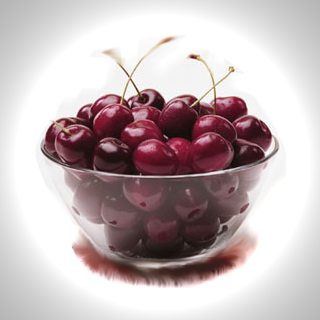
\includegraphics[width=0.33\textwidth]{figures/radiometric_before.png}}
  \subfigure[]{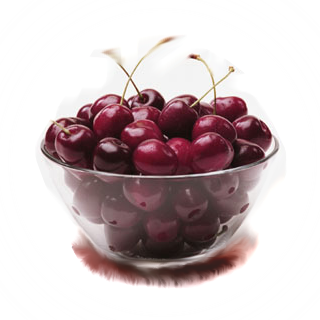
\includegraphics[width=0.33\textwidth]{figures/radiometric_after.png}}
 \end{center}
 \caption{
  Przykład zniekształceń radiometrycznych:
  (a) obraz zniekształcony;
  (b) obraz skorygowany.
 }
 \label{fig:radiometric}
\end{figure}